\textbf{SHIFT}

First I implemented and tested Gaussian blur.

\begin{figure}[H]
    \centering
    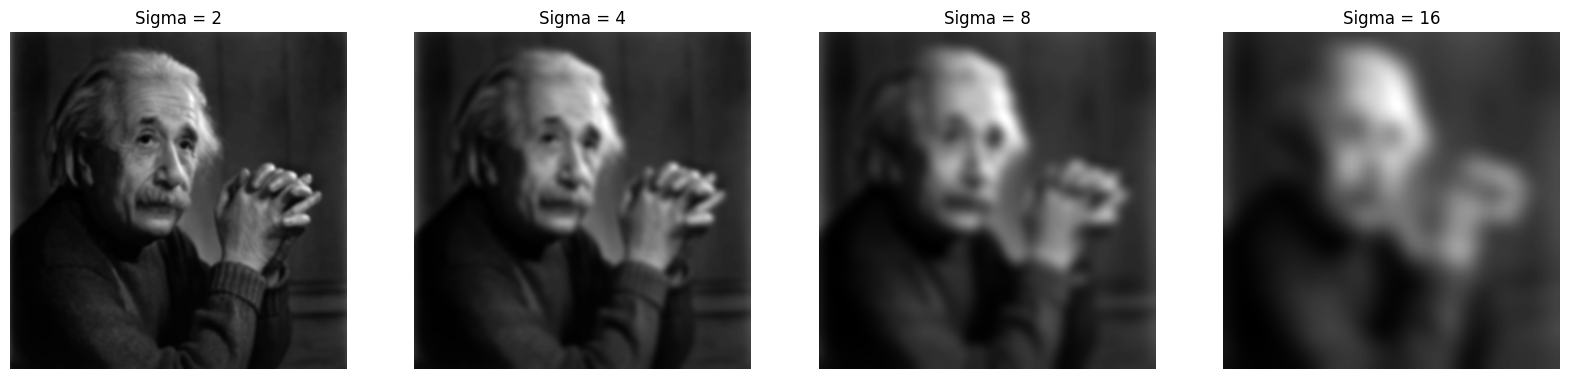
\includegraphics[width=1\textwidth]{res/blur.png}
    \caption{Gaussian blur with different sigma values}
    \label{fig:1.1}
\end{figure}

Then I computed the \textbf{SIFT keypoints} in the image. The keypoints are shown in the image below. The method to compute the keypoints is as follows:

\textbf{Parameters:}

\begin{enumerate}
    \item \textit{Inital sigma} the base sigma for the Gaussian kernel.
    \item \textit{Octaves} the number of octaves in the image. For each octave, the image is downsampled by a factor of 2 and the initial sigma multiplied by two.
    \item \textit{Scales} the number of scales in each octave. The number of scales is the number of times the image is blurred with a Gaussian kernel.
    \item \textit{Threshold} the threshold for the difference of Gaussian (DoG) image. If the difference of two consecutive scales is greater than the threshold, the pixel is considered a keypoint.
\end{enumerate}

\textbf{Algorithm:}

\begin{enumerate}
    \item First create a Gaussian pyramid. For each octave, there will be a list of blurred images.
    \item Compute the difference of Gaussian (DoG) images. For each octave, there will be a list of DoG images.
    \item Compute the keypoints. For each octave, there will be a list of keypoints.
\end{enumerate}

\begin{figure}[H]
    \centering
    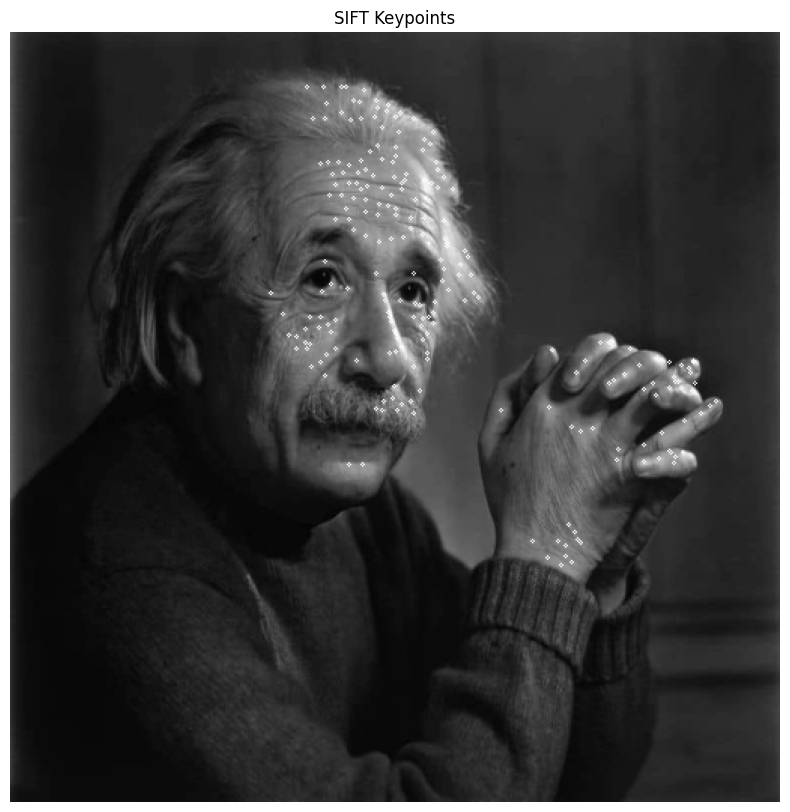
\includegraphics[width=.33\textwidth]{res/sift_keypoints.png}
    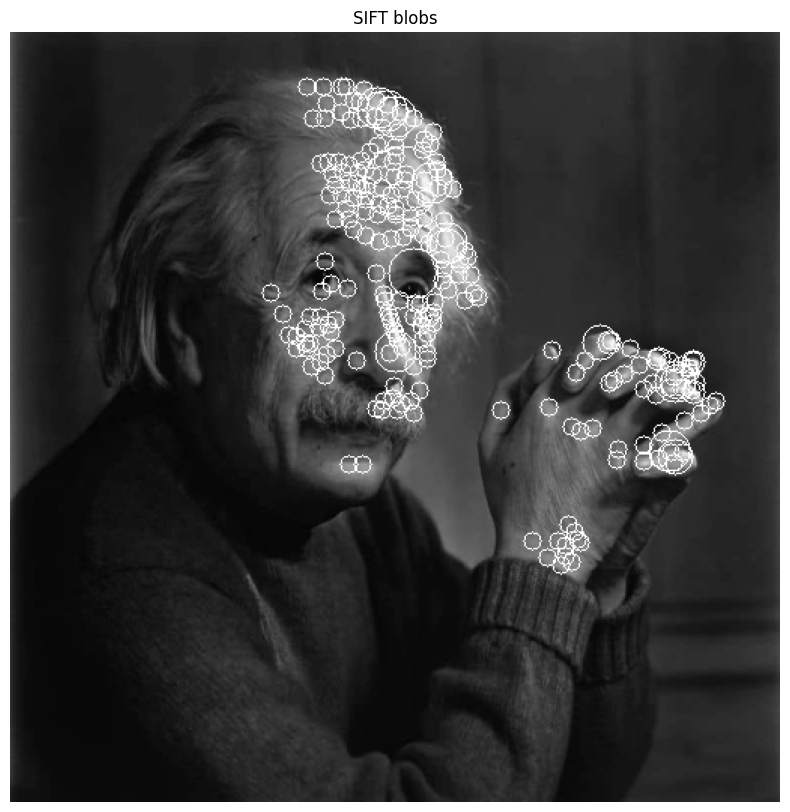
\includegraphics[width=.33\textwidth]{res/sift_blobs.png}
    \caption{SIFT keypoints and blobs}
    \label{fig:1.2}
\end{figure}


\newpage

\textbf{Bag of Words}

For Bag of Words, I have randomly sampled few 8x8 patches from the main image. Now these are my words. To match them and extract the feature vector, I have used l2 norm to find the distance between the patches. The feature vector is the histogram of the patches. The histogram is the frequency of each patch in the image. The feature vector is then can be used to classify the image.

\begin{figure}[H]
    \centering
    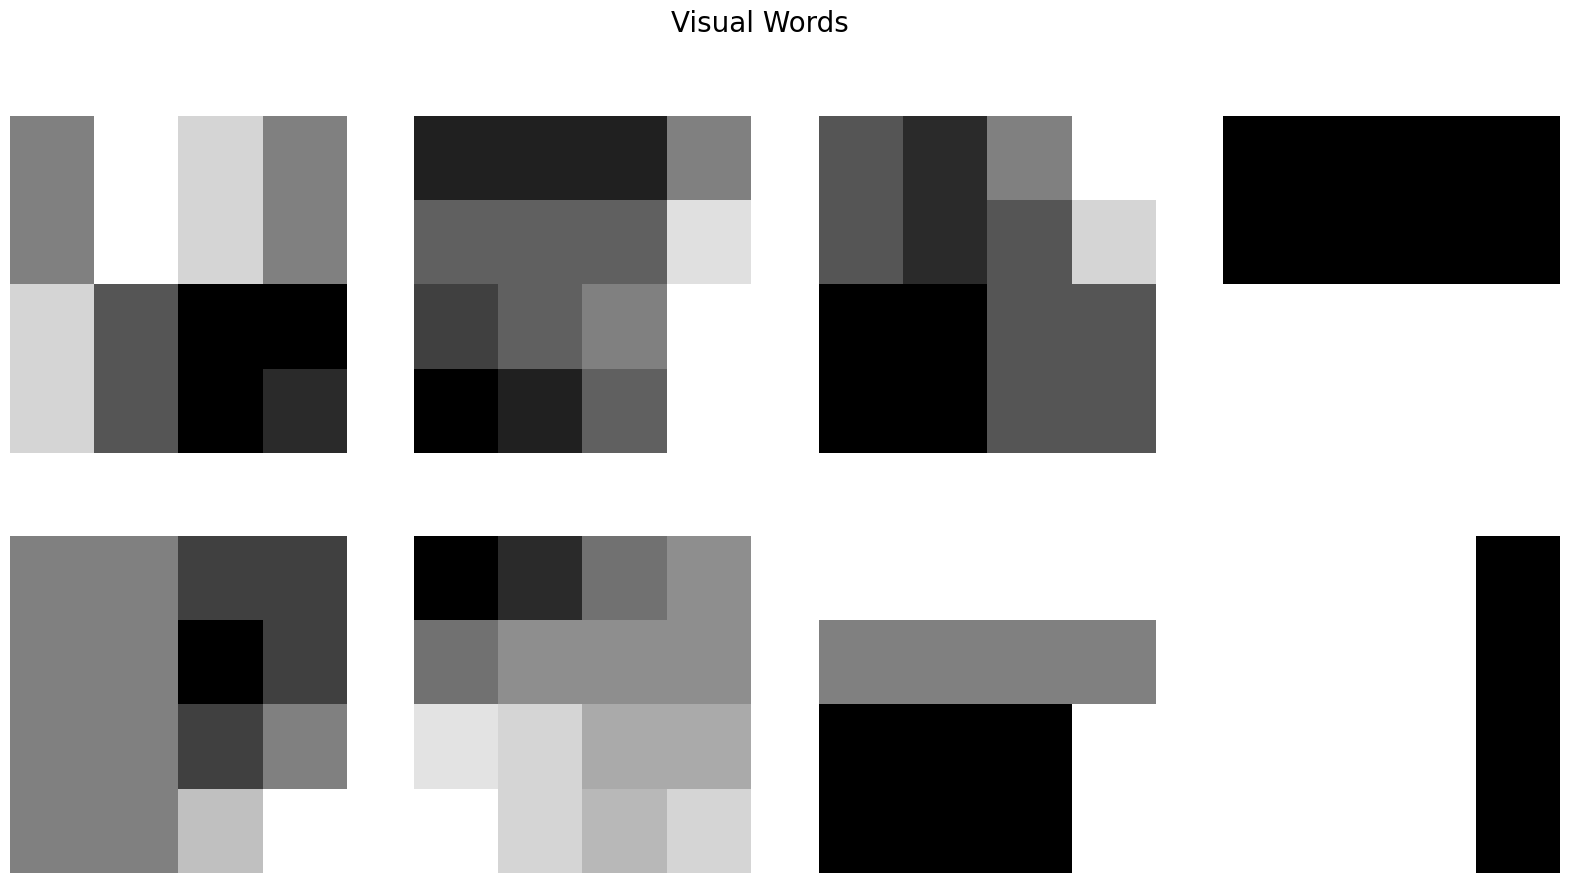
\includegraphics[width=1\textwidth]{res/bow_patches.png}
    \caption{Bag of Words patches}
    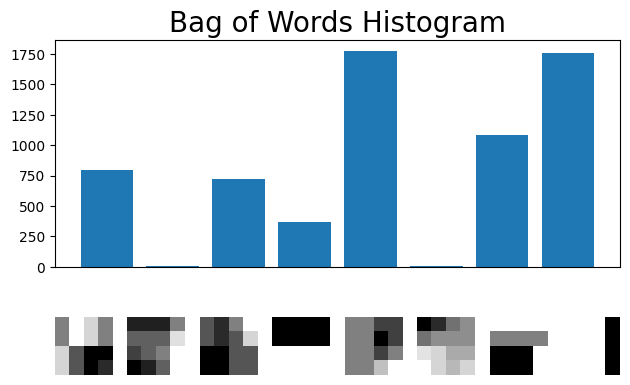
\includegraphics[width=1\textwidth]{res/bow_hist.png}
    \caption{Bag of Words histogram}
    \label{fig:1.3}
\end{figure}


\newpage

\textbf{HOG}

For HOG, I have computed the gradient of the image. The gradient is then divided into cells. The cells are then divided into blocks. The histogram of the gradient is computed for each block. The histogram is then normalized. The normalized histogram is then concatenated to form the feature vector.

\begin{figure}[H]
    \centering
    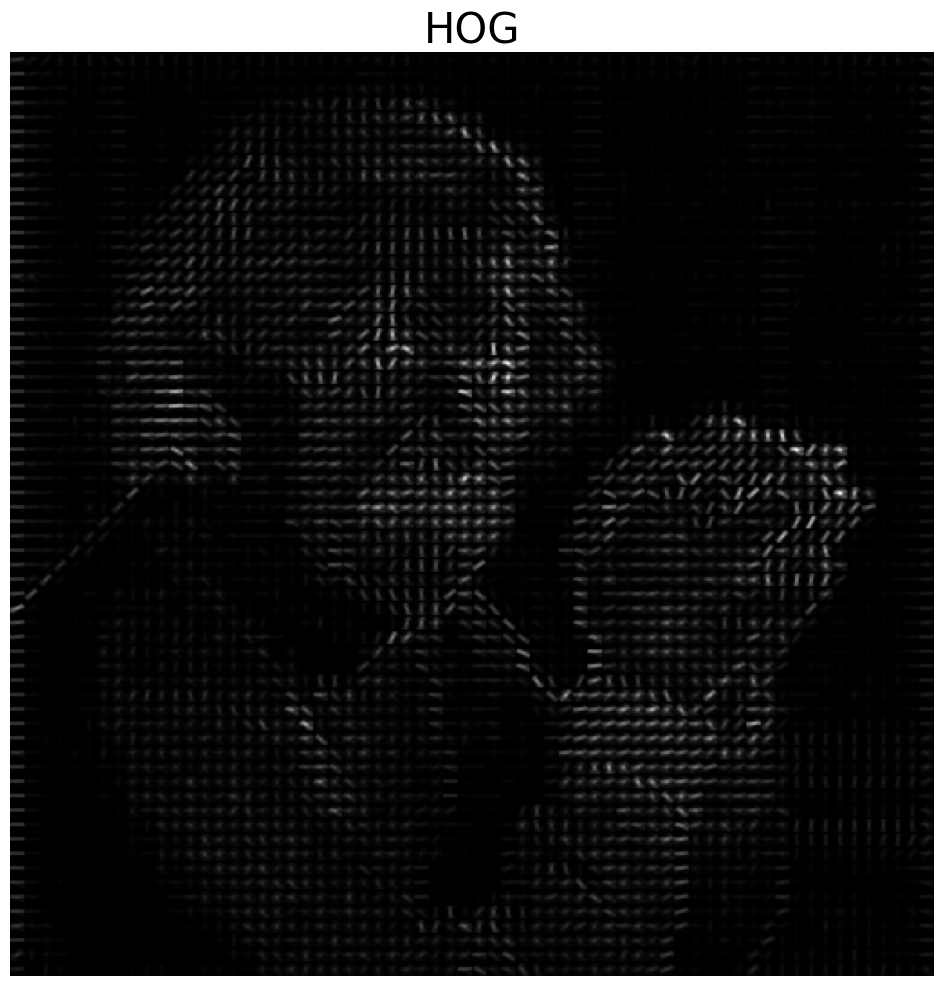
\includegraphics[width=.6\textwidth]{res/chog.png}
    \caption{C-HOG Image}
    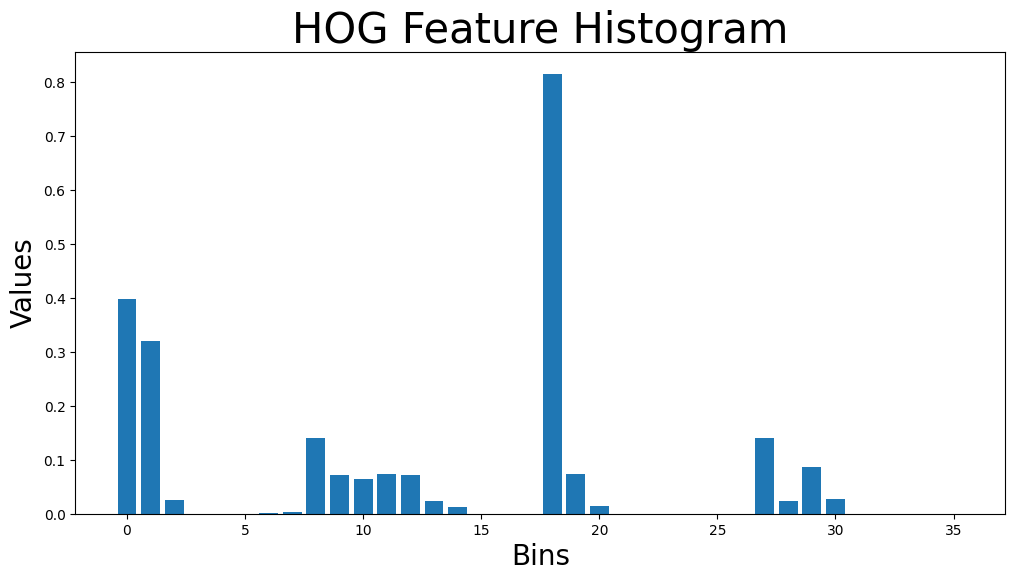
\includegraphics[width=.9\textwidth]{res/hog_feature.png}
    \caption{HOG feature}
    \label{fig:1.4}
\end{figure}